\documentclass[a4paper]{report}
\usepackage[utf8]{inputenc}
\usepackage[portuguese]{babel}
\usepackage{hyperref}
\usepackage{a4wide}
\hypersetup{pdftitle={AP - Poisson},
pdfauthor={João Teixeira, José Ferreira},
colorlinks=true,
urlcolor=blue,
linkcolor=black}
\usepackage{subcaption}
\usepackage{listings}
\usepackage{booktabs}
\usepackage{multirow}
\usepackage{appendix}
\usepackage{tikz}
\usepackage{authblk}
\usepackage{bashful}
\usepackage{verbatim}
\usepackage{amssymb}
\usepackage{multirow}
\usepackage{mwe}
\usepackage[parfill]{parskip}
\usetikzlibrary{positioning,automata,decorations.markings}
\AfterEndEnvironment{figure}{\noindent\ignorespaces}
\AfterEndEnvironment{table}{\noindent\ignorespaces}

\begin{document}

\title{Algoritmos Paralelos\\Numerical Solution of the Poisson Equation}
\author{João Teixeira (A85504) \and José Filipe Ferreira (A83683)}
\date{\today}

\begin{center}
    \begin{minipage}{0.75\linewidth}
        \centering
        
\includegraphics[width=0.4\textwidth]{images/eng.jpeg}\par\vspace{1cm}
        \vspace{1.5cm}
        \href{https://www.uminho.pt/PT}
        {\color{black}{\scshape\LARGE Universidade do Minho}} \par
        \vspace{1cm}
        \href{https://www.di.uminho.pt/}
        {\color{black}{\scshape\Large Departamento de Informática}} \par
        \vspace{1.5cm}
        \maketitle
    \end{minipage}
\end{center}

\tableofcontents

\pagebreak

\chapter{Introdução}
A equação de Poisson é usada nas áreas das ciências naturais e da física
teórica. A solução desta equação pode ser usada para, por exemplo, simular os
campos electromagnéticos gerados por partículas electricamente carregadas. Esta
é uma generalização da equação de Laplace que também tem múltiplos usos na
física teórica.

A formulação desta equação a duas dimensões e dada por:

\[ \left( \frac{\partial^2 u}{\partial x^2} + \frac{\partial^2 u}{\partial y^2} \right)= g(x, y) \]

Para simplificar assume-se que g(x,y) = 0 sendo que u representa o limite da
área. Os valores da solução não são computados de forma continua mas sim de
forma discreta.

Ao longo deste relatório iremos descrever os vários algoritmos iterativos
desenvolvidos em C com o objetivo de aproximar a solução desta equação assim
como a estratégia de paralelização utilizada com vista a melhorar a performance
dos mesmos culminando numa analise de tempos de execução.

\chapter{Algoritmos Desenvolvidos}

Foram desenvolvidos três algoritmos iterativos distintos para resolver este
problema. Gauss-Seidel, Gauss-Seidel com Red-Black e Successive Overrelaxation
com Red-Black.

Todos os algoritmos recebem como parâmetro o tamanho do vetor a resolver e o
valor de tolerância e devolvem o vetor com os valores aproximados e o numero de
iterações que tiveram de ocorrer para calcular esse valor.

O vetor que contem o que foi calculado até ao momento denomina-se de w e o vetor
que contem o que foi calculado na iteração anterior denomina-se de u. O vetor w
é populado no inicio com todos os valores na borda com o valor 100, menos na
borda superior em que os valores são 0, e com os valores interiores iguais a 50.

Numa primeira tentativa de melhorar a performance do algoritmo, paralelizou-se o
ato de popular a matriz. Visto que o algoritmo inicial já vetorizava

Para todos os algoritmos o caso de paragem consiste em subtrair o vetor w com o
u e procurar qual é o valor maior em modulo. Esse modulo é comparado com o valor
de tolerância passado por argumento. Caso o valor de tolerância seja maior do
que o valor calculado então o algoritmo iterativo  acaba.

Desta forma, a única diferença entre estes algoritmos na sua forma sequencial
encontra-se na forma como eles percorrem e calculam o vetor w em cada iteração.

\section{Gauss-Seidel}

O algoritmo de Gauss-Seidel consiste em percorrer todos os pontos do vetor w
linha por linha. Para cada ponto soma-se o ponto que está diretamente acima, o
ponto abaixo, o ponto à esquerda e o ponto à direita e divide-se o resultado por
4. Desta forma o valor do ponto é substituído pela média dos pontos diretamente
adjacentes.

% TODO explicar paralelização

\section{Gauss-Seidel com Red-Black}

Tal como se viu o algoritmo de Gauss-Seidel simples não é fácil de
paralelizar. Por isso, foi criado uma versão modificada do algoritmo que
percorre o vetor w de forma diferente para tentar mitigar este problema.

O método utilizado de percorrer o vetor é conhecido como Red-Black porque o
resultado se assemelha a um tabuleiro de xadrez com as casas de cor vermelha e
preta. Dentro de cada iteração primeiro percorre-se posição sim posição não de
cada linha par e posição não posição sim de cada linha par (células vermelhas da
imagem \ref{fig:chess}) e depois percorre-se posição não posição sim de cada
linha par e posição sim posição não de cada linha ímpar (células pretas da
imagem \ref{fig:chess}). Em cada iteração, para cada uma das posições do vetor w
o novo valor é dado na mesma por calcular a média dos pontos diretamente
adjacentes

\begin{figure}[h]
    \centering
        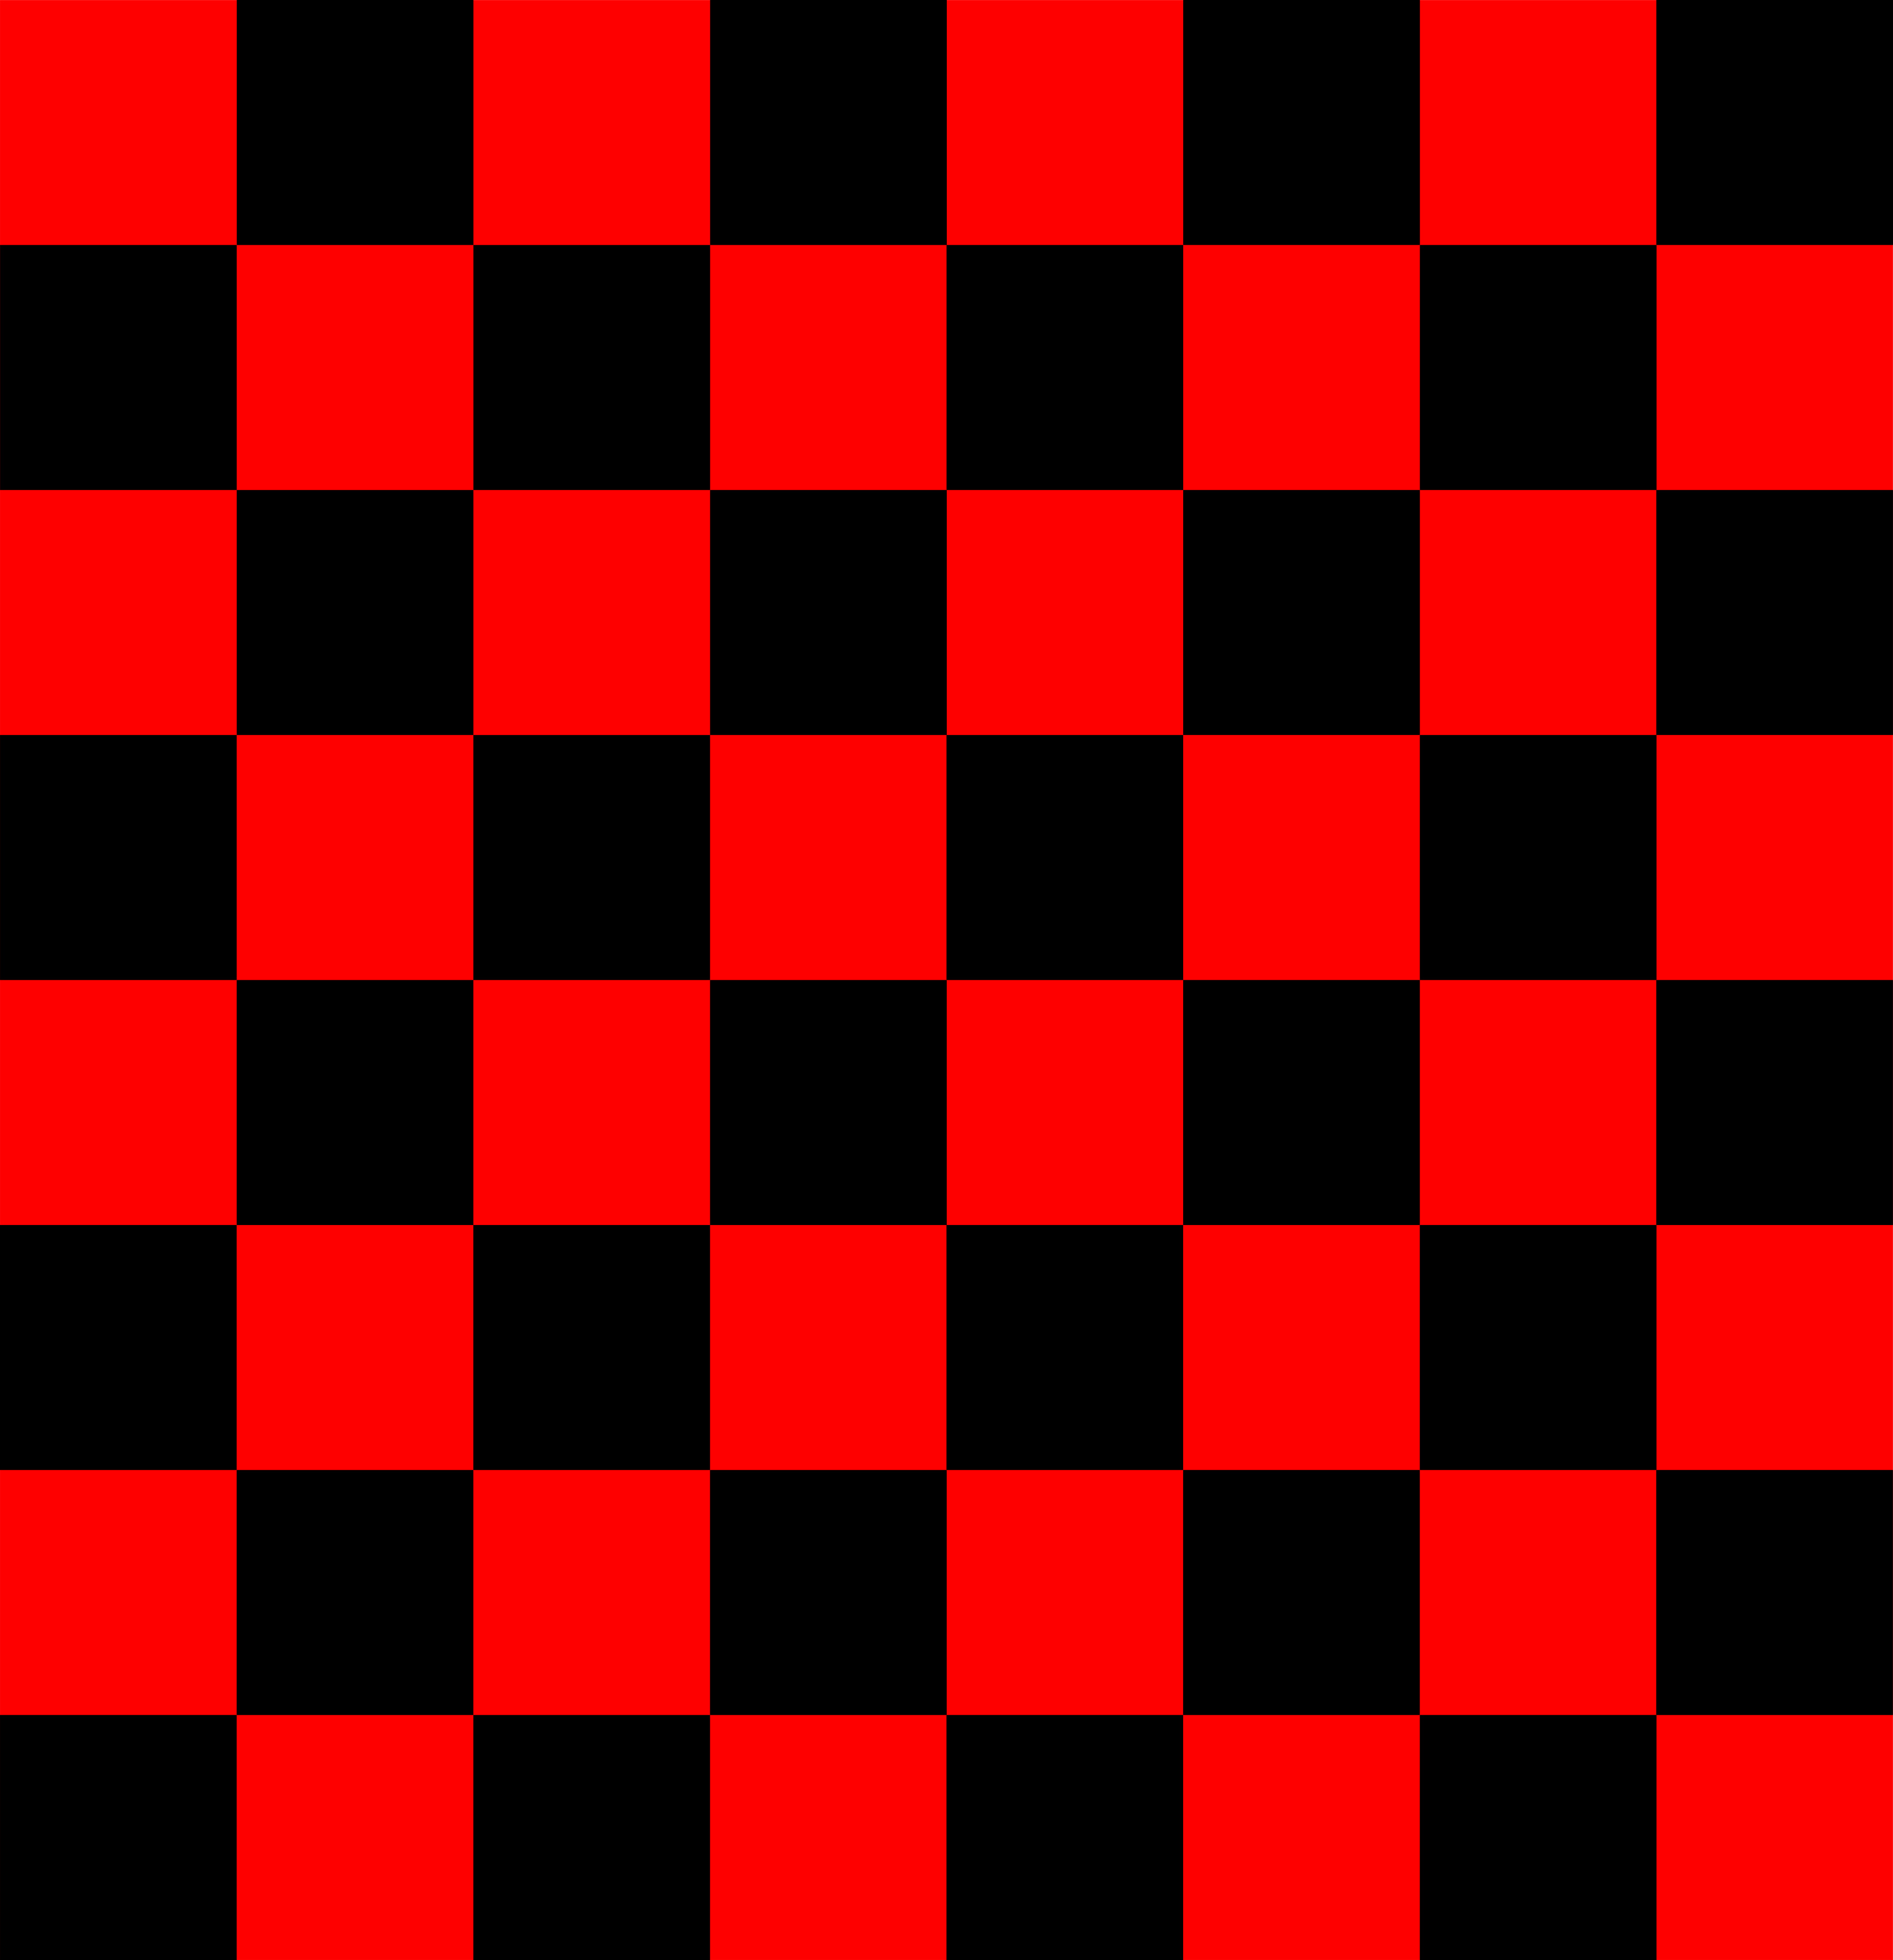
\includegraphics[width=0.4\textwidth]{images/chess.jpg}
        \caption{tabuleiro de xadrez}
        \label{fig:chess}
\end{figure}

Desta forma cada uma destas duas passagens dentro de cada iteração não tem
dependências de dados dentro de si mesmas.

% TODO explicar paralelização

\section{Successive Overrelaxation com Red-Black}

A versão sequencial deste algoritmo é muito próxima da versão sequencial do
algoritmo Gauss-Seidel com Red-Black. No Successive Overrelaxation com Red-Black
o que difere é a parte como é calculado o novo valor do vetor w. Neste caso,
para além de se ter em conta a média dos quatro pontos adjacentes ao ponto que
se está a calcular, também se tem em conta o próprio valor seguindo a formula:

\[ p = \frac{2}{1 + sin{\frac{\pi}{SIZE - 1}}} \]
\[novo\_valor = (1-p) * pixel + p * media \]

Esta mudança implica que o algoritmo tende mais rapidamente para o caso de
paragem e, por isso, tende a ter menos iterações.

% TODO explicar paralelização

\chapter{Representação de Resultados}

Para representar os resultados obtidos pelos algoritmos criados, foi feita uma
função que representa o vetor w sobre a forma de uma imagem no formato
\textit{portable pixmap format} (PPM). Este formato foi escolhido devido ao
facto de suportar formato ASCII tornando a escrita da imagem substancialmente
mais simples. O formato indica que existem duas áreas no ficheiro. Uma primeira
área que indica o formato utilizado e uma segunda área com os pontos
propriamente ditos.

A área do formato contem três linhas. A primeira linha representa o formato em
que a imagem foi escrita. Neste caso o formato escolhido foi o formato P3 que
indica que a imagem está escrita em ASCII e que representa pontos RGB. A segunda
linha indica as dimensões da imagem separada por espaço. Por fim, a ultima linha
representa o valor máximo de cada valor de cor. Neste caso o valor escolhido
foi 255.

A área com os pontos propriamente ditos contem um ponto por linha. Sendo que
cada linha contem o valor R, o valor G e o valor B do pixel separado por espaços.

Desta forma, para representar uma imagem com apenas um pixel branco basta fazer:
\begin{verbatim}
P3
1 1
255
255 255 255
\end{verbatim}

Para representar os pontos do vetor estes são primeiro convertidos para HSV.
Neste passo a Saturação e Valor são sempre mantidos constantes para todos os
pontos, sendo que o único valor que varia é o Hue. Para existir uma variação
constante de azul para amarelo com o aumento dos valores é necessário que o Hue
varie entre 60 e 240. O próximo passo consiste em converter os valores dentro do
vetor w para estarem contidos dentro desse intervalo. Por fim pode-se converter
o HSV obtido para RGB e colocar no ficheiro.

\begin{figure}[h]
\centering
\begin{minipage}{.3\textwidth}
  \centering
  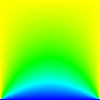
\includegraphics[width=.95\linewidth]{images/poisson_gs_100.png}
\end{minipage}%
\begin{minipage}{.3\textwidth}
  \centering
  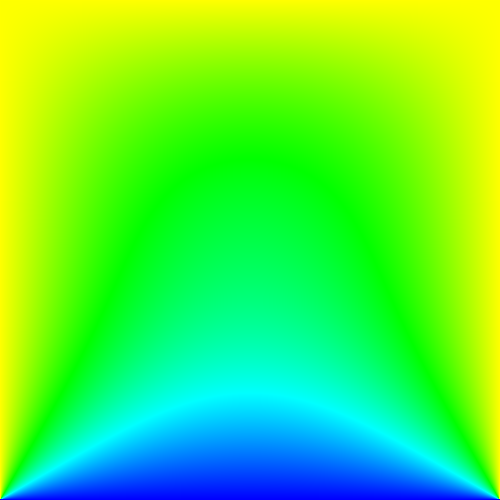
\includegraphics[width=.95\linewidth]{images/poisson_gs_500.png}
\end{minipage}
\begin{minipage}{.3\textwidth}
  \centering
  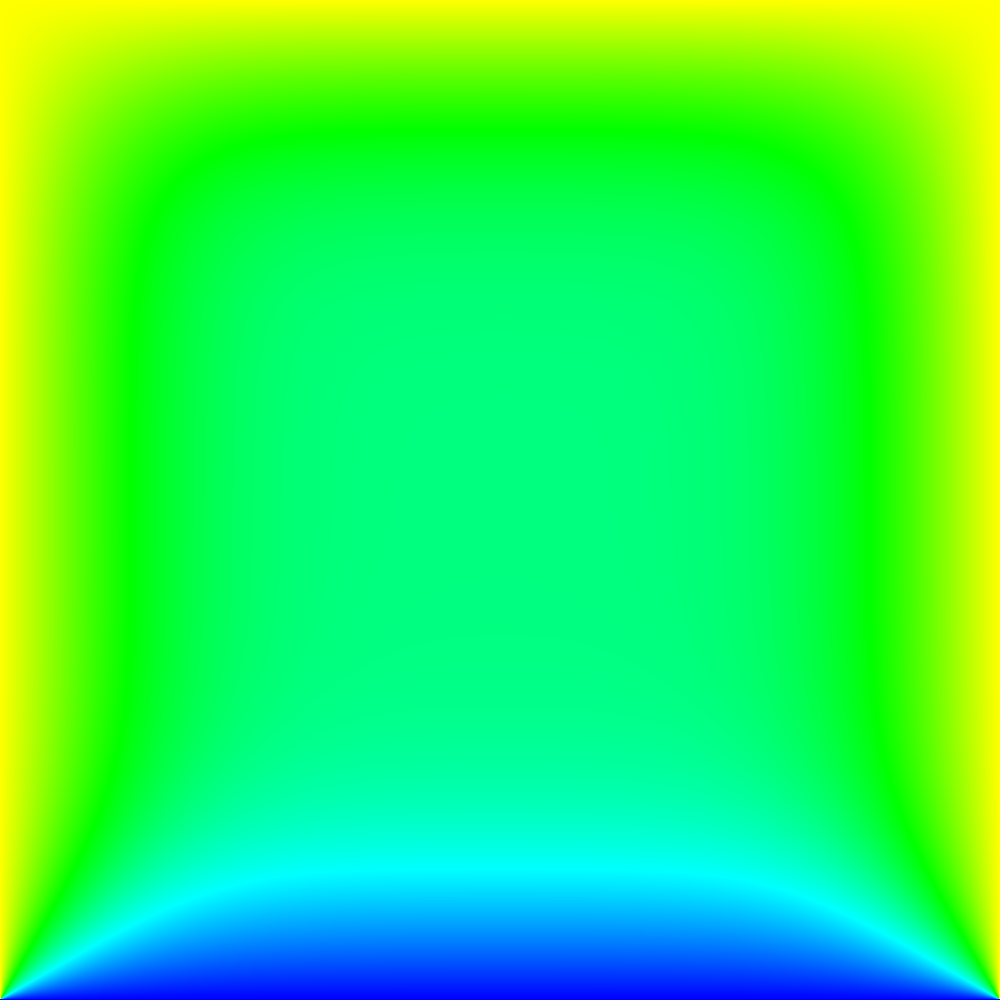
\includegraphics[width=.95\linewidth]{images/poisson_gs_1000.png}
\end{minipage}
    \caption{Comparação de diferentes outputs com diferentes tamanhos e
    tolerância constante}
\end{figure}

\chapter{Analize de Resultados}

Os testes foram corridos no cluster Search da universidade do Minho nas máquinas
da fila cpar, nomeadamente as máquinas 652. Os valores foram obtidos fazendo uso
do k-best com k igual a 8. O programa foi compilado com -O3.


\begin{table}[h]
\centering
\begin{tabular}{|l|l|l|}
\hline
                                                 & num iterações & tempo (segundos) \\ \hline
Gauss-Seidel                                     & 922           & 0.050               \\ \hline
Gauss-Seidel paralelo                            & 922           & 135.080               \\ \hline
Gauss-Seidel com Red-Black                       & 540           & 0.020               \\ \hline
Gauss-Seidel com Red-Black paralelo              & 915           & 1.720               \\ \hline
Successive Overrelaxation com Red-Black          & 571           & 0.010               \\ \hline
Successive Overrelaxation com Red-Black paralelo & 571           & 0.280               \\ \hline
\end{tabular}
\caption{Comparação de Performance (para N=100 e TOL=0.001)}
\label{tab:tempo}
\end{table}

\begin{table}[h]
\centering
\begin{tabular}{|l|l|l|}
\hline
                                                 & num iterações & tempo (segundos) \\ \hline
Gauss-Seidel                                     & 923           & 1.670            \\ \hline
Gauss-Seidel paralelo                            & 923           & 516.480          \\ \hline
Gauss-Seidel com Red-Black                       & 610           & 0.440               \\ \hline
Gauss-Seidel com Red-Black paralelo              & 902           & 23.270               \\ \hline
Successive Overrelaxation com Red-Black          & 126           & 0.460            \\ \hline
Successive Overrelaxation com Red-Black paralelo & 126           & 14.660           \\ \hline
\end{tabular}
\caption{Comparação de Performance (para N=500 e TOL=0.001)}
\label{tab:tempo}
\end{table}

\begin{table}[h]
\centering
\begin{tabular}{|l|l|l|}
\hline
                                                 & num iterações & tempo (segundos) \\ \hline
Gauss-Seidel                                     & 922           & 7.030            \\ \hline
Gauss-Seidel paralelo                            & 922           & 1189.080         \\ \hline
Gauss-Seidel com Red-Black                       & 610           & 2.140                 \\ \hline
Gauss-Seidel com Red-Black paralelo              & 902           & 153.540                 \\ \hline
Successive Overrelaxation com Red-Black          & 1107          & 3.870            \\ \hline
Successive Overrelaxation com Red-Black paralelo & 1107          & 123.730          \\ \hline
\end{tabular}
\caption{Comparação de Performance (para N=1000 e TOL=0.001)}
\label{tab:tempo}
\end{table}

\end{document}
